\chapter{Convertitore Tensione-Frequenza}

%--------------------------------------------------------------------------------------------

Si vuole ora progettare la sezione per la generazione del segnale di clock, con le specifiche
ottenute dal capitolo precedente, ovvero:

\begin{itemize}
    \item Frequenza minima: $\approx 14kHz$;
    \item Frequenza massima: $\approx 3.6MHz$;
    \item Livello logico basso: $0V$;
    \item Livello logico alto: $+5V$;
\end{itemize}

%--------------------------------------------------------------------------------------------

\subsection*{Principio di Funzionamento}

%--------------------------------------------------------------------------------------------

Ciò di cui abbiamo bisogno è un circuito in grado di convertire una tensione in un segnale
a onda quadra con frequenza proporzionale alla tensione stessa, ovvero un convertitore
tensione-frequenza.

In commercio è possibile trovare chip in grado di svolgere questa funzione con l'aggiunta
di una manciata di componenti di contorno, anche se la maggior parte di questi non
arriva a coprire l'intero range di funzionamento di cui abbiamo bisogno (come ad esempio
il noto LM331 \cite{lm331}). Nel nostro caso si utilizza un VFC110 \cite{vfc110},
circuito integrato che vanta un'ottima linearità e in grado di arrivare a fornire una
frequenza in uscita di $4MHz$ in corrispondenza di una tensione di ingresso di $10V$,
esattamente ciò che la nostra applicazione richiede.
\medskip

\begin{figure}[ht]
    \centering
    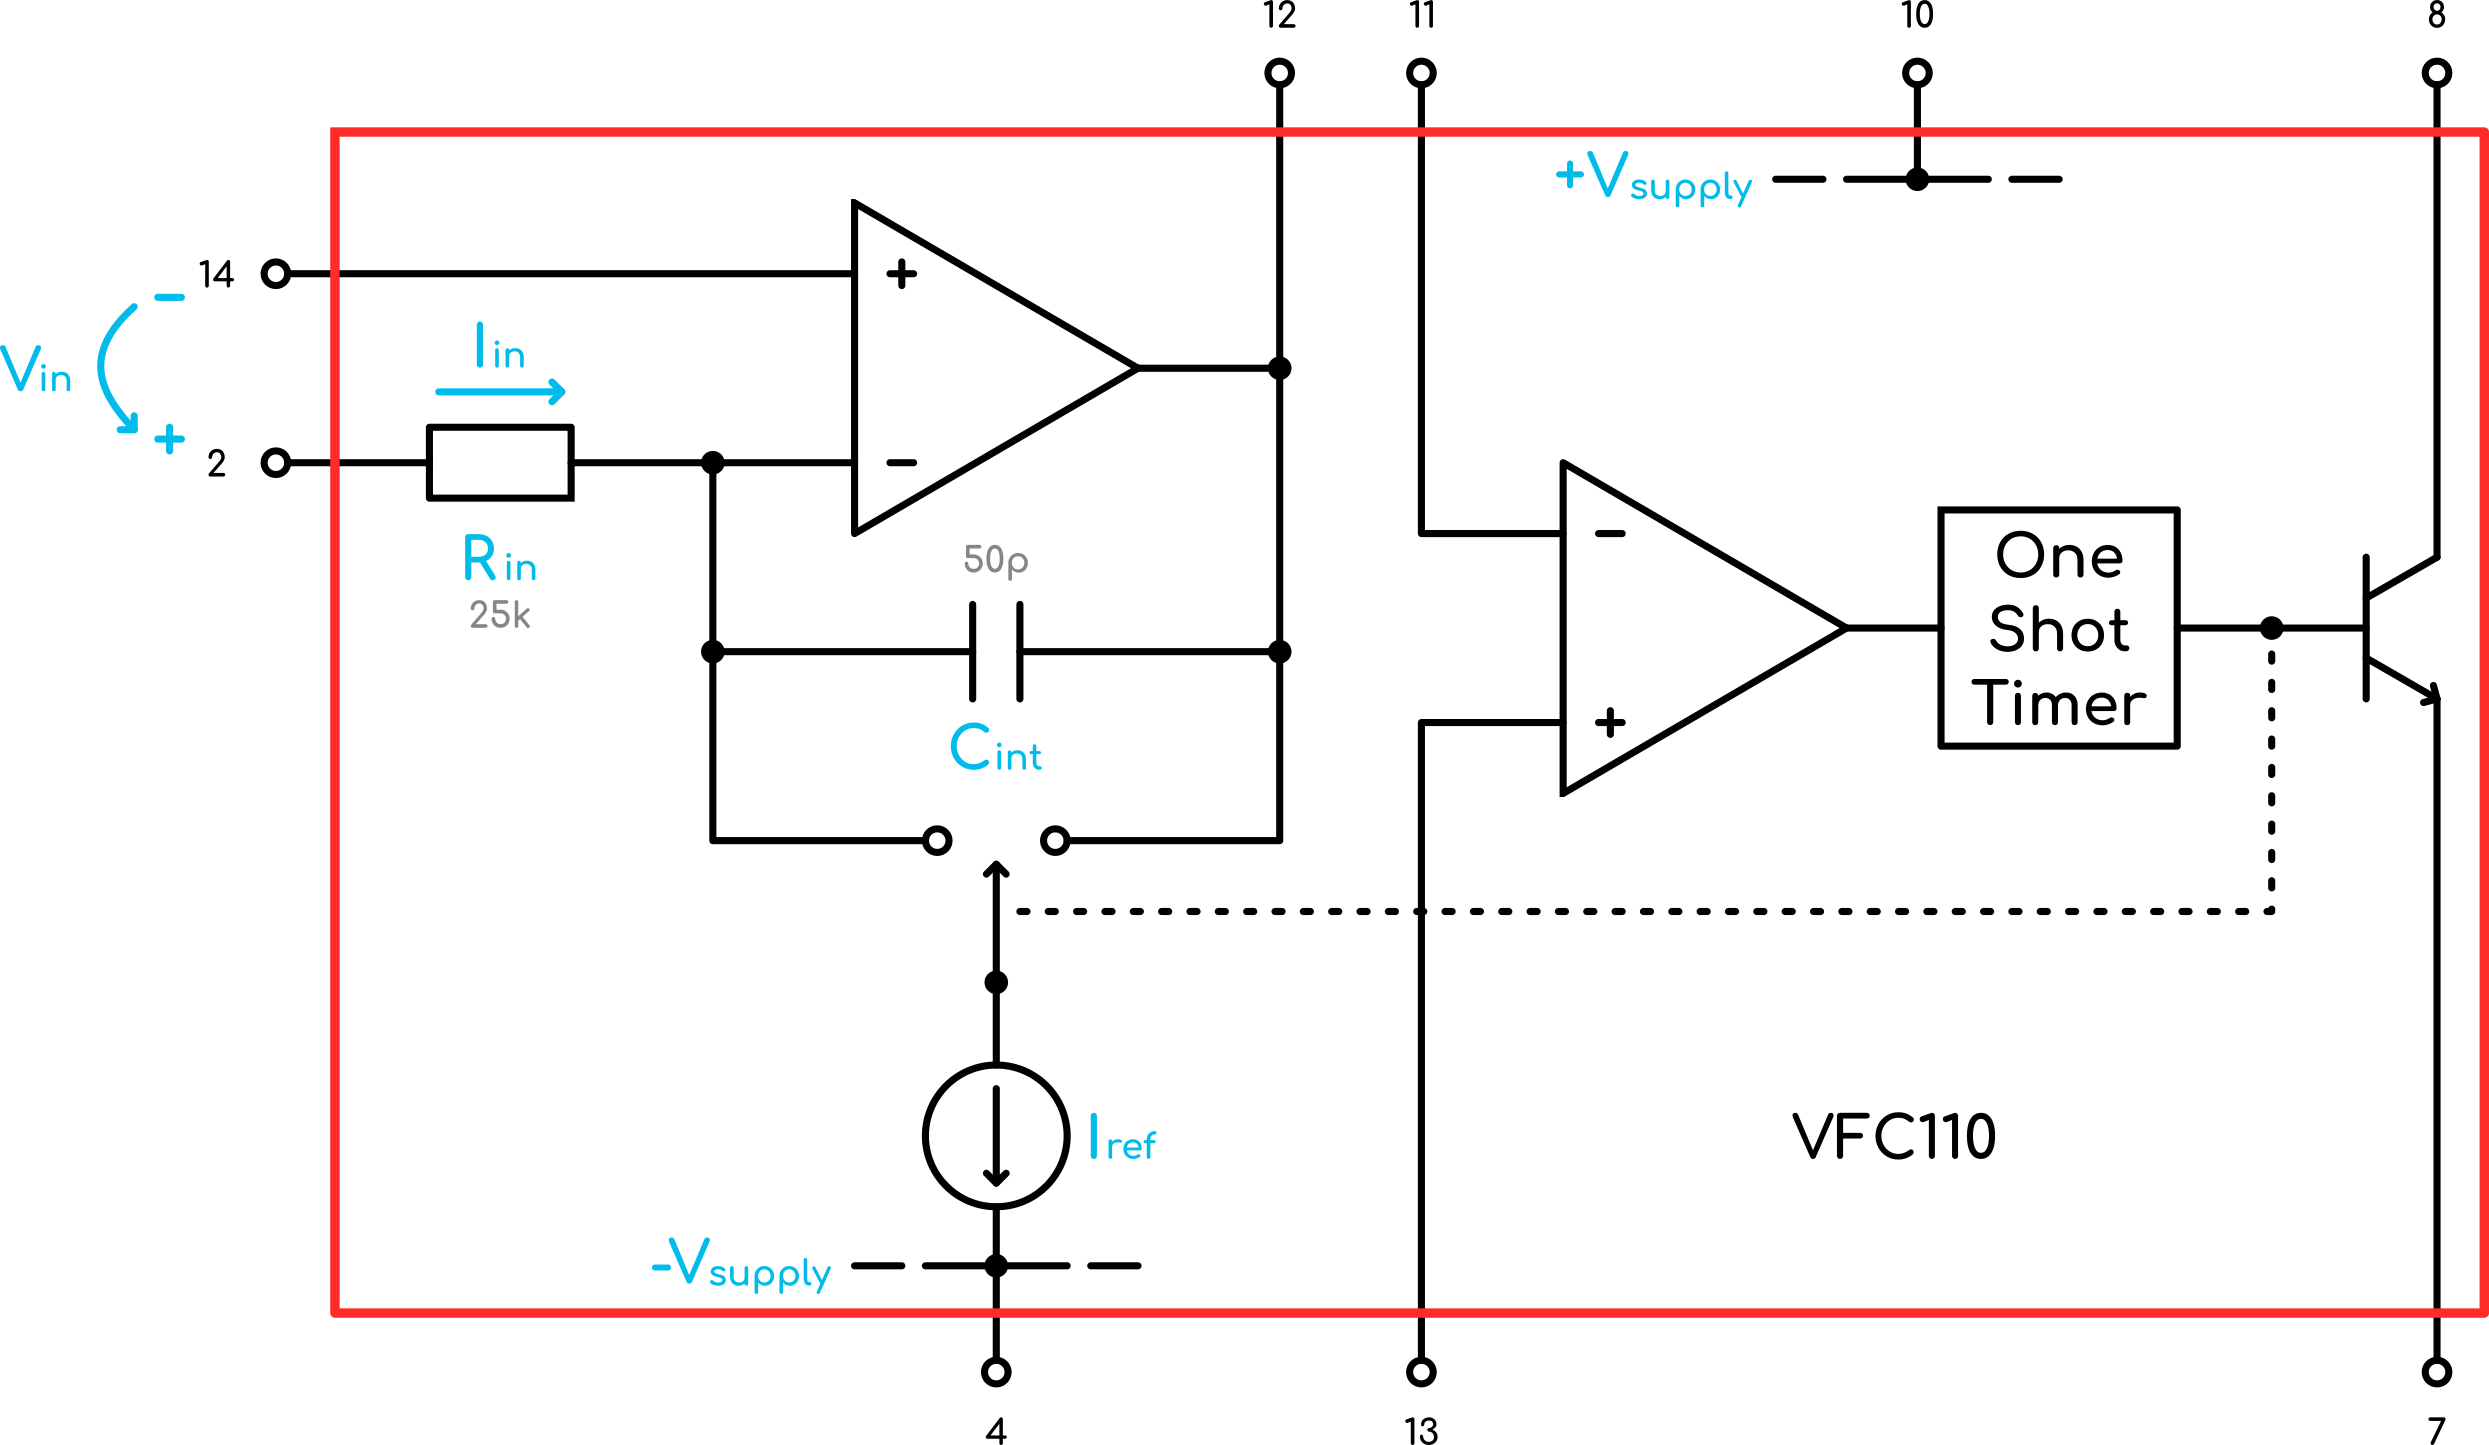
\includegraphics{circuits/vfc110_internal.png}
    \caption{Estratto della struttura interna di un VFC110}
    \label{vfc100_internal}
\end{figure}

Il circuito fa uso di un integratore, la quale uscita è proporzionale alla carica immagazzinata
in $C_{int}$. Una tensione in ingresso $V_{in}$ sviluppa una corrente $I_{in}=\frac{V_{in}}{R_{in}}$
e che viene forzata in $C_{int}$, caricandolo e causando l'uscita dell'integratore a diminuire
linearmente. Non appena l'uscita dell'integratore arriva a $0V$, il comparatore scatta, attivando
il timer one-shot. Quindi un generatore di corrente $I_{ref}$ (circa $1mA$) viene connesso
all'uscita dell'integratore durante il periodo del timer $T_{OS}$ causando l'uscita dell'integratore
a crescere linearmente fino alla fine di $T_{OS}$. Successivamente il ciclo ricomincia.

L'oscillazione è regolata dall'equilibrio tra corrente in ingresso $I_{in}$ e la corrente di
reset media.
\medskip

\begin{figure}[ht]
    \centering
    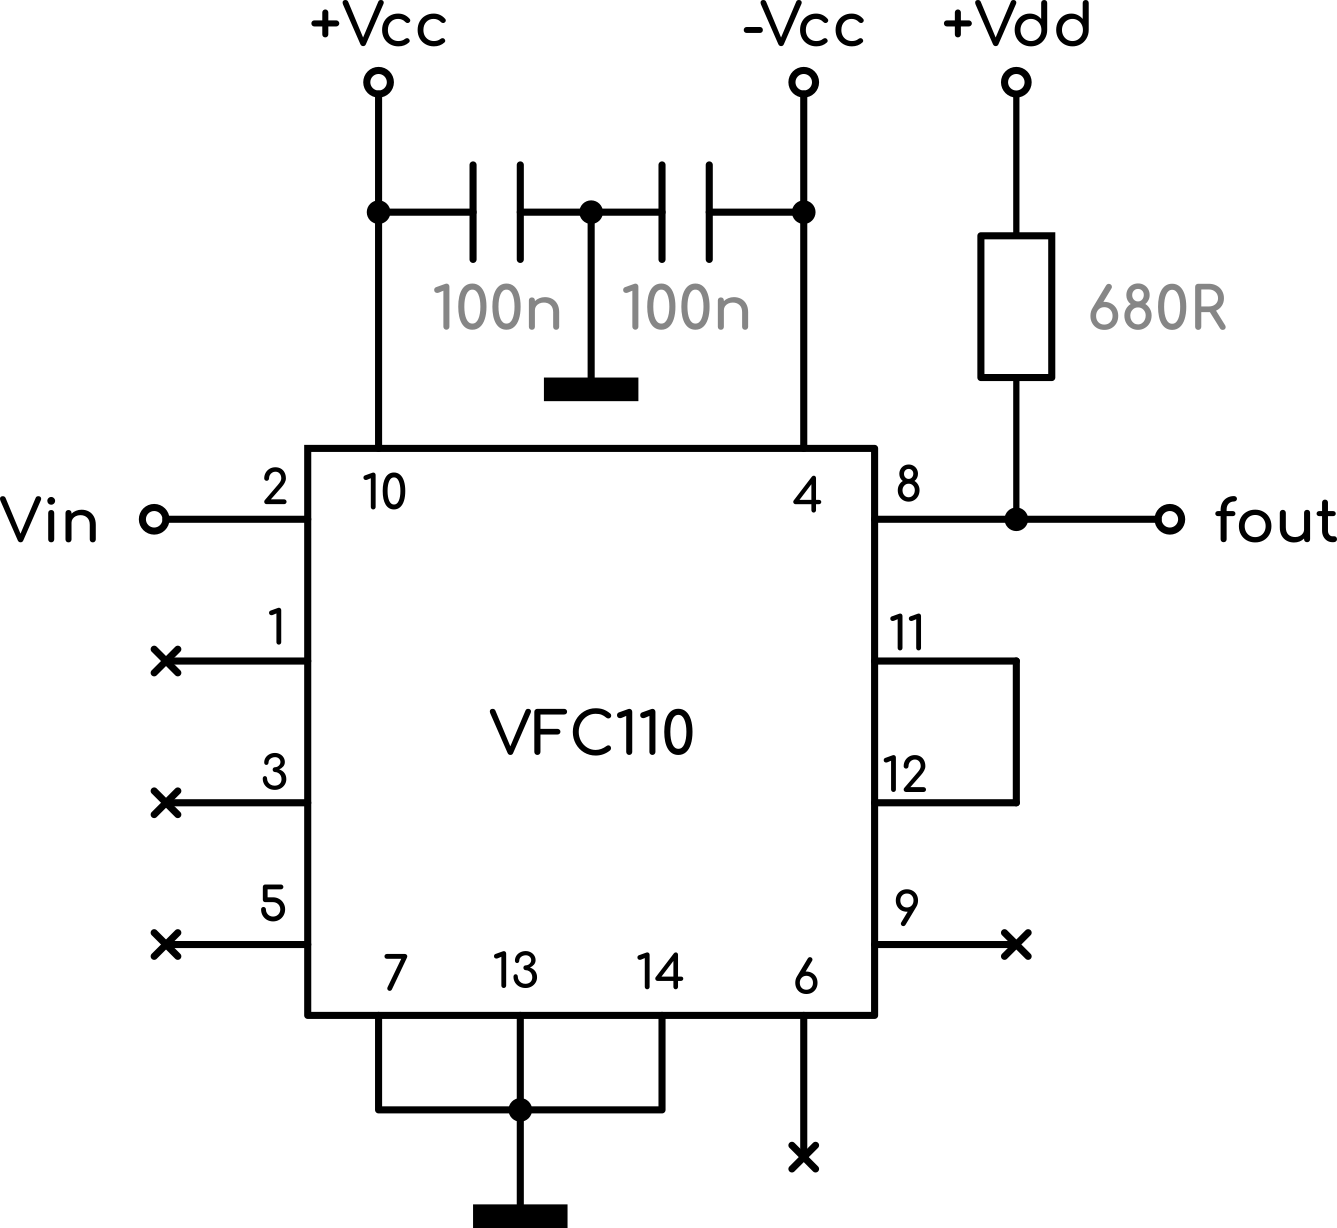
\includegraphics{circuits/VFC_circuit.png}
    \caption{Schema elettrico del VFC110 utilizzato}
    \label{VFC_circuit}
\end{figure}

Per uno studio più approfondito sul funzionamento del componente si rimanda al datasheet
del componente, dal quale si ricava anche la configurazione del circuito da utilizzare
per sfruttare l'intero range offerto, modificando però i valori di alimentazione con
quelli dello standard scelto ($\pm 12V$).
\medskip

% schema elettrico

Si noti che gli unici componenti aggiunti sono condensatori di filtro e un resistore di
pull-up per l'uscita a collettore aperto.

Le relazioni tra le grandezze in gioco sono le seguenti:

$$
    I_{in}=I_{ref}\cdot\delta
    \rightarrow
    \delta=\frac{I_{in}}{I_{ref}}=\frac{V_{in}}{R_{in}\cdot I_{ref}}
$$

$$
    \frac{V_{in}}{R_{in}}=I_{ref}\cdot f_{out}\cdot T_{OS}
    \rightarrow
    f_{out}=\frac{V_{in}}{R_{in}\cdot I_{ref}\cdot T_{OS}}=\frac{\delta}{T_{OS}}
$$

%--------------------------------------------------------------------------------------------

\subsection*{Risultati Pratici e Misure}

%--------------------------------------------------------------------------------------------

% grafica setup di misura

\begin{figure}[ht]
    \centering
    
\includegraphics{misc/oscilloscope_placeholder.png}
    \caption{Acquisizione dell'uscita dell'integratore (pin 12) e $f_{out}$ corrispondente}
    \label{acq_vfc110}
\end{figure}

% misura di Tos

% grafico V_in/duty (misurato e teorico) e tabella valori
% grafico V_in/f_out (misurato e teorico) e tabella valori
